\chapter{Compression on the basis of equivalence classes}

\section{Related Compression Techniques}
Compression of sequencing short reads becomes crucial with the lowering cost of sequencing technology. The rapid technological development enables the generation of petabytes of data on servers worldwide. Apart from size, often succinct representation \citep{Pritt2016} also yields almost accurate results with a much smaller memory footprint. Nucleotide sequence compression can largely be divided into two paradigms, one is reference based compression where the reference is needed to transfer to the decoder end along with the compressed data ~\citep{Canovas2014}, \citep{Fritz2011}, \citep{Li2014}. Another is reference free compression, \citep{adjeroh2002dna},\citep{Bonfield_2014}, \citep{Hach2012} where the read sequences are compressed independent of reference sequence, barring the burden of transferring reference. Such compressions are commonly known as \Denovo compression. A robust and widely used \denovo compressor, LEON \citep{Benoit2015}, constructs a de Bruijn graph from the k-mer counts table extracted build on the reads. Reads are then mapped to the newly constructed de Bruijn graph, and are stored in form of anchor address, read size and bifurcation list.   

Reference based compressions start with the BAM file produced by state of the art aligners such as \Bowtie. Typically these algorithms store the edits after aligning the sequences to reference. \citet{Fritz2011} is one such widely used tool A serious bottleneck of such approaches is to store all meta information in the BAM file which can be regenerated re-aligning the reads to the provided reference sequence. This problem is partially addressed by fastq \citep{bonfield2013compression}, where a new alignment technique is being implemented to navigate through the problem of storing meta-data footprint. 

\begin{figure}[!ht]
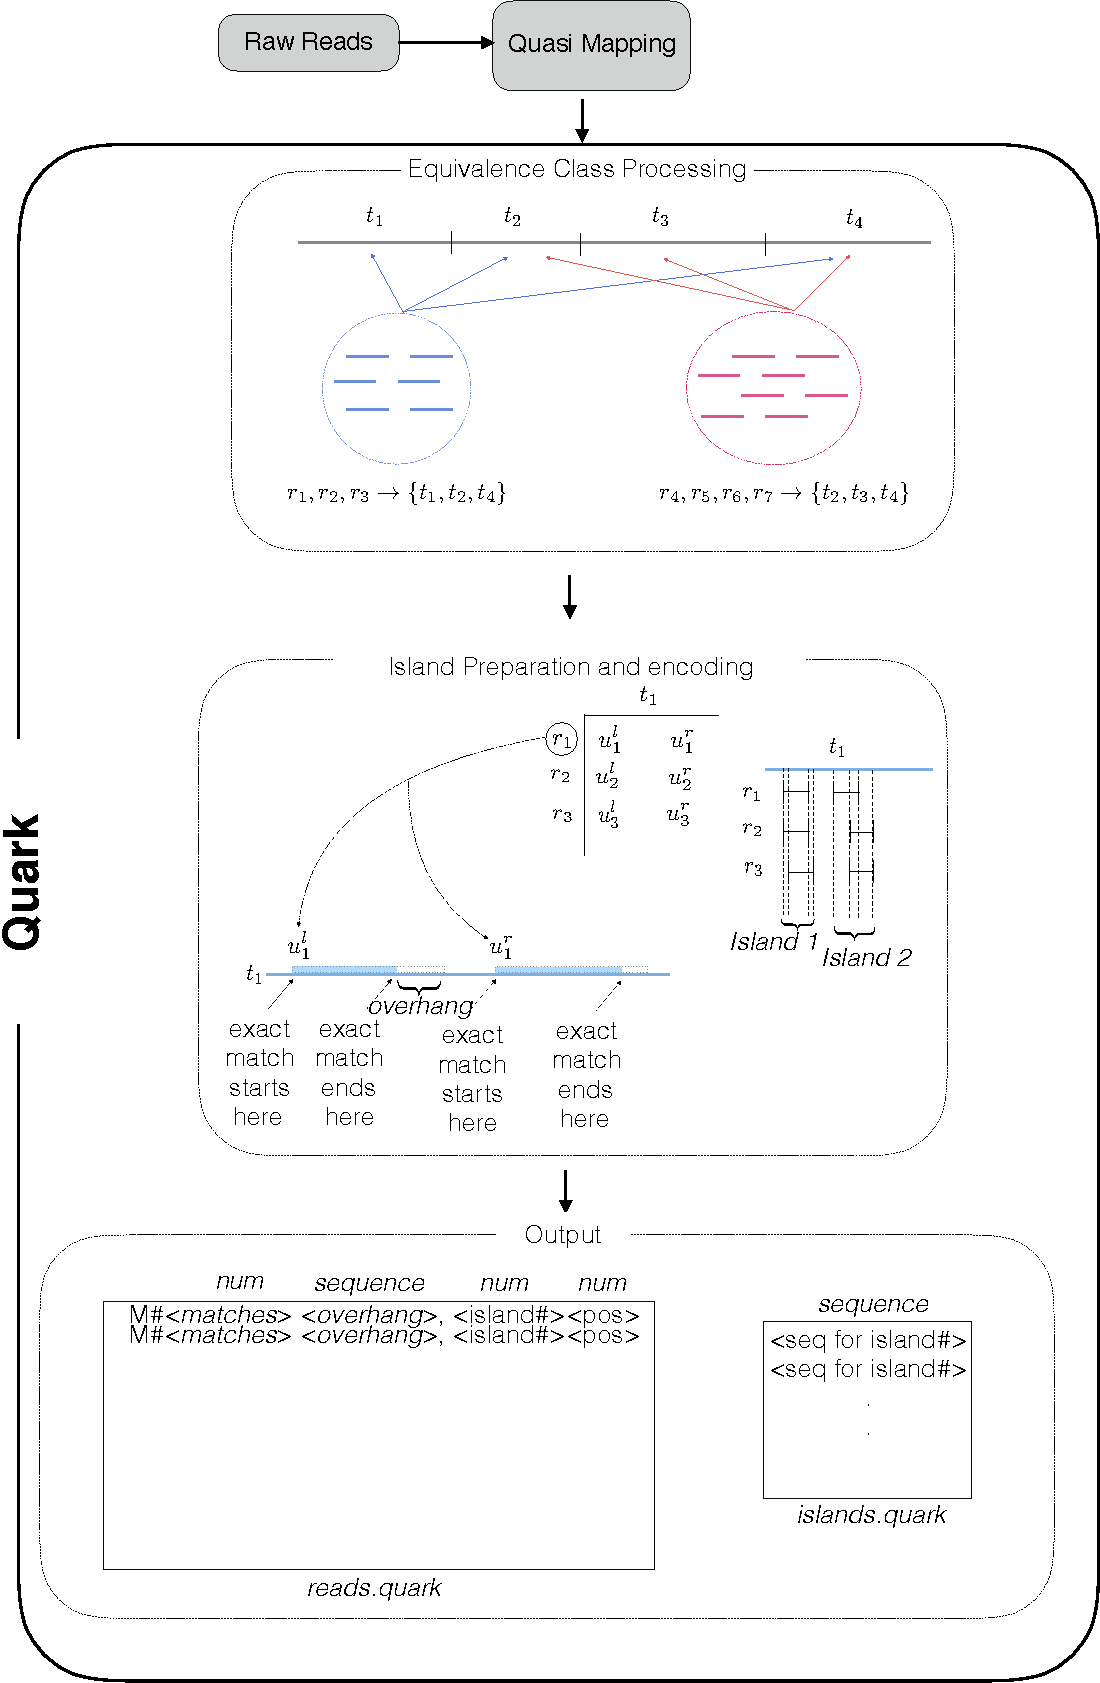
\includegraphics[width=\textwidth]{Figures/quark_overview4-crop}
\centering
\caption{\label{fig:overview_quark}An overview of the \quark pipeline. Equivalence classes are computed using \qm, Reads within classes along with the positions are then used find out the exact match length and the overhang portion. Islands are simultaneously processed from the intervals. In the last steps encoded reads along with the islands are stored as \quark output.}
\end{figure}


There are few mappers which does compression of genome/transcriptome for the better mapping, and also compress reads on the way. Recently published CORA ~\citep{Yorukoglu2016} is a compressive read mapper. The working principle of CORA is interesting and worth mentioning as concept of equivalence classes is also used there, but carries a different meaning. CORA converts the fastq reads to non redundent k-mer sets. Furthermore, CORA does a redundancy removal on reference genome, by self mapping. The positions where a k-mer maps form an equivalence class. Two equivalence classes are regarded as concordant if all positions of one equivalence class are in one nucleotide shift distance from another equivalence class. 

Apart from reference based and \denovo mappers, few mappers lie in the middle, which  stores a part of the reference that is shared between reads. Kpath \citep{Kingsford2015} is a tool that stores the shared reference as that acts as a backbone for a statistical generative model. An arithmetic coding is performed on the reads.

In the current chapter we would present a semi-reference mapper \quark which takes the raw reads and transcripts from the user and perform a \qm on it. The mapping information is then utilized to represent the reads. The motivation for such a scheme comes from the observation of the fact that, thee are some parts of a particular transcript which are over abundant, therefore storing the entire transcriptome is almost useless. A decoder on the other end takes the parts of the transcript we refer as \iss and compressed reads to produce the uncompressed data. An overview of \quark is given in \fref{fig:overview_quark}. The method section is divided into three parts, in the heart of \quark, \qm maps the raw reads to the indexed transcriptome and reports the position of the exact matched k-mer. In the next step we collect the position and the target transcripts and later merged the boundaries to yield a set of \iss. We would go over the method in greater detail in \sref{sec:quark_method}

\section{Method}\label{sec:quark_method}
At a conceptual level \quark exploits the mapping principle used in \qm, therefore it is worth going over the basic mechanism of \qm adopted from \citet{rapmap}. In \fref{fig:overview_quasi} the basic steps of \qm is described. \Qm starts with a matched \kmer that is shared between a transcript and read sequence. If such a match exists, \qm tries to extend the match further by searching the interval of the suffix array for a maximal matched prefix. 

 
\begin{figure}[!ht]
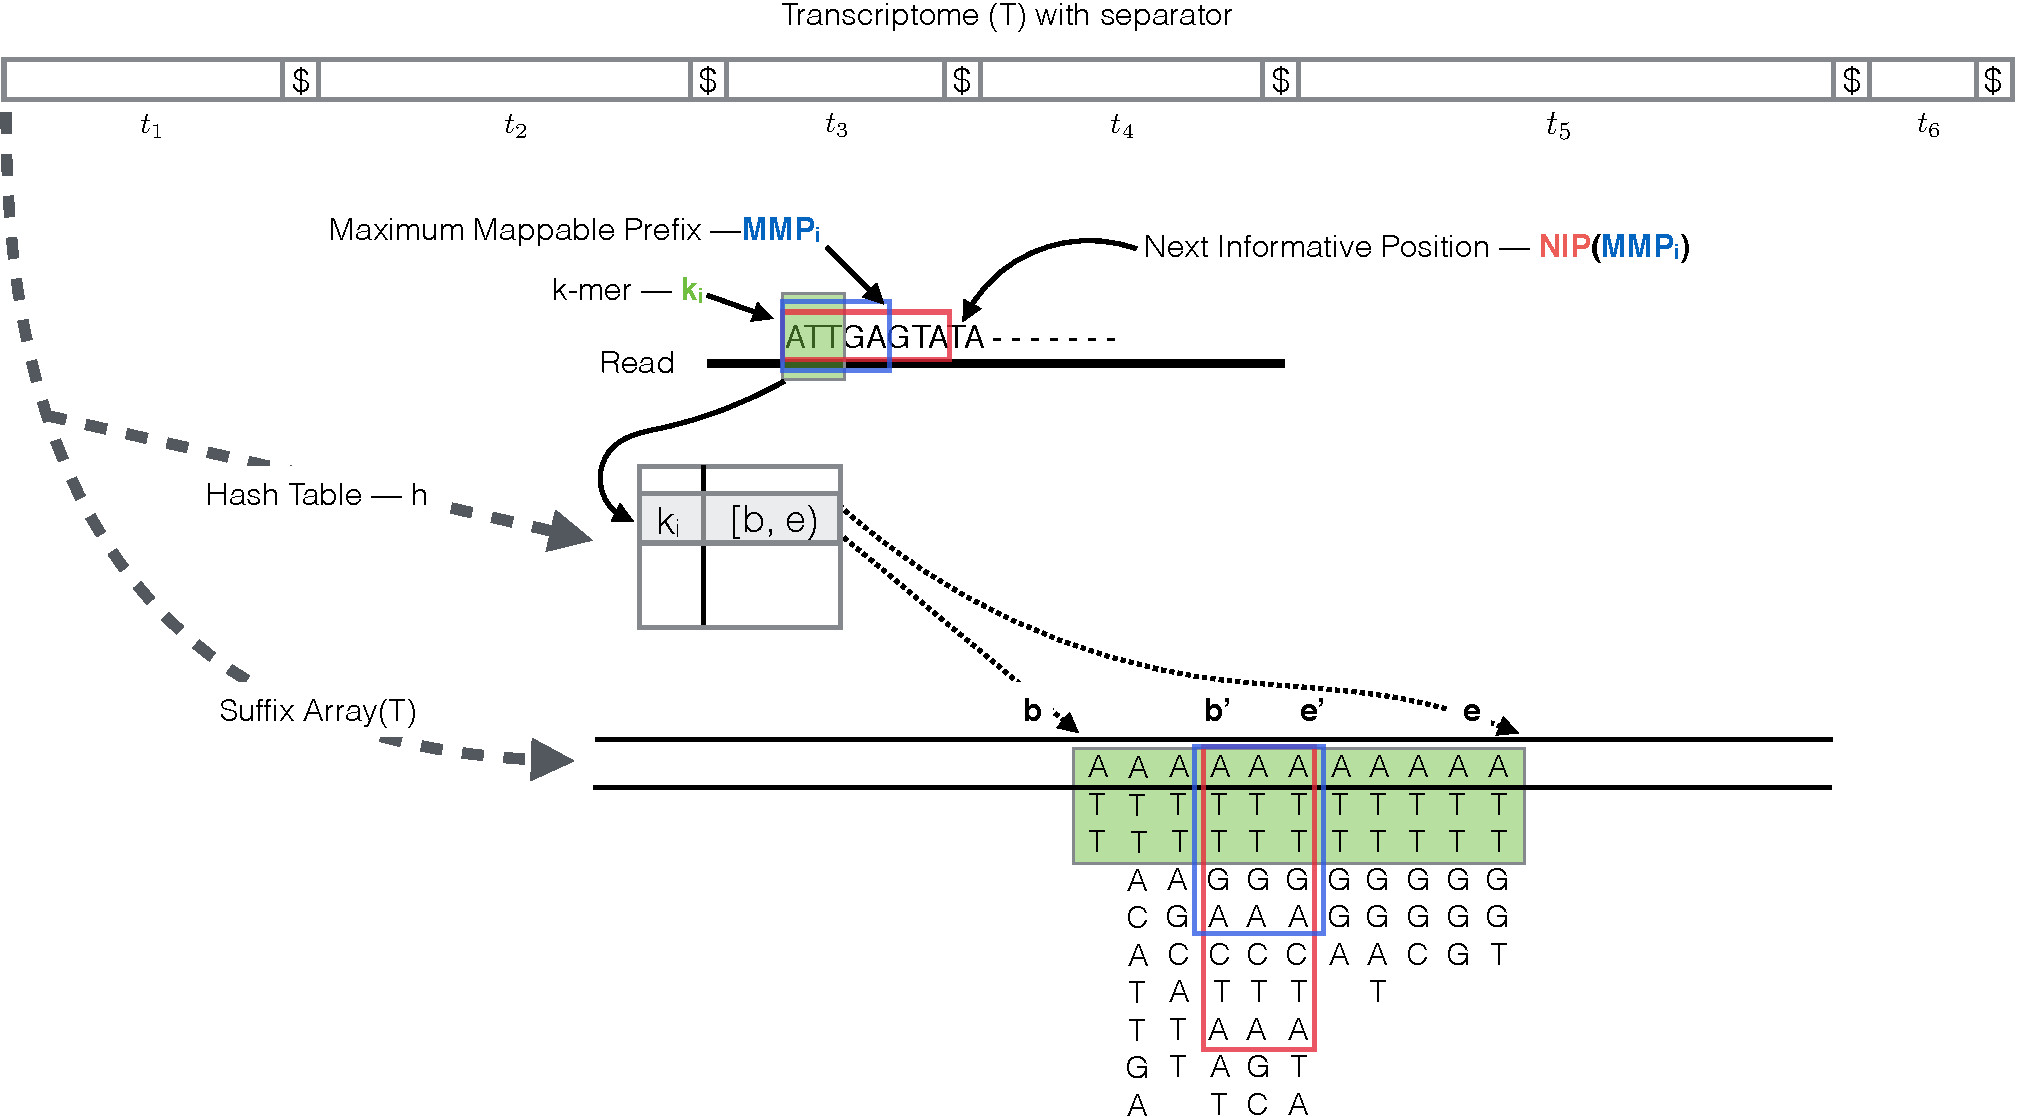
\includegraphics[width=\textwidth]{Figures/overview_quasi}
\centering
\caption{\label{fig:overview_quasi}The transcriptome (consisting of transcripts $t_1,\ldots ,t_6$) is converted into a $\$$-separated string, $T$, upon which a suffix array of T, and a hash table, $h$, are constructed. The mapping operation begins with a \kmer (here, $k=3$) mapping to an interval $\{b,e\}$ in suffix array of T.}
\end{figure}

We divide the \textit{quasi-mapped} reads into three categories, 
\begin{itemize}
    \item \it{Mapped reads:} If both the reads of the mate pair get mapped. This is ideal situation where we can encode both the ends most efficiently. Because each of the read at least shares a \kmer.
    \item {Orphan reads:} For reads in this category we can not map both ends of the mate pair. In \quark we keep the orphan or unmapped end as it is.
    \item {Unmapped reads:} There is not a single \kmer that is shared between reference  and read.
\end{itemize}

Given the above result in \quark we follow a hierarchical structure, where the mapped reads are distributed into equivalence classes according to \sref{subsec:gen_equiv_classes}. Knowing the fact that all reads in equivalence classes share at least a \kmer with the reference transcript and each other. The encoding scheme itself is straight forward. Given the position and the reference sequence, we do a linear search on the reference sequence to find out the maximal match. This search is guaranteed to yield a match of at least $31$ nucleotides given the criterion of \qm.

\subsection{Forming Islands}

Formation of \iss are very similar to what we see in de bruijn graphs. Given the intervals on the reference sequence, that might share some nucleotides we merge the intervals to form disjoint \iss. As shown in \fref{fig:overview_quark} the encoded reads are assigned to an \is id. The use of \is comes to aid in terms of the compression factor. To study the effectiveness of constructing \iss we considered dataset SRR635193. After mapping to gencode reference transcript, we observe that out of 95309 transcripts only 49589 transcripts are used by \quark. Moreover as shown in \fref{fig:ratio}, there are a lot of transcripts where only a small fraction of nucleotides are used as islands.  

\begin{figure}[!ht]
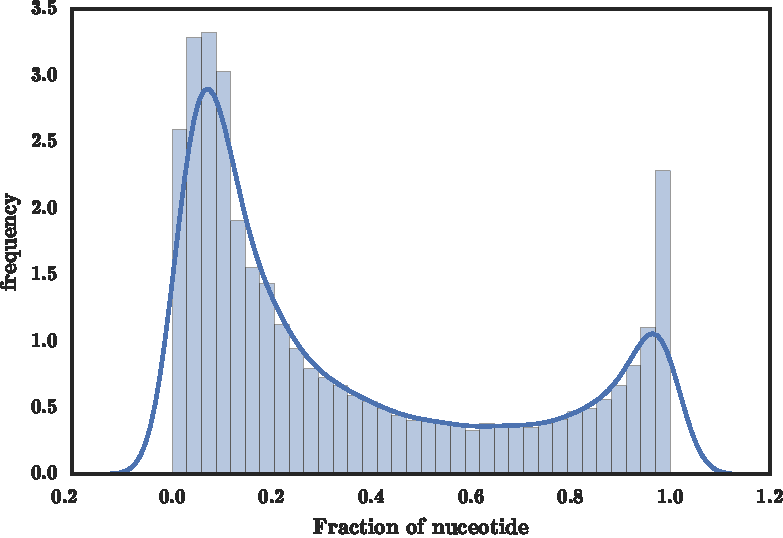
\includegraphics[width=0.5\textwidth]{Figures/ratio}
\centering
\caption{\label{fig:ratio}Islands consist of only a fraction of nucleotides of expressed transcripts}
\end{figure}

\subsection{Post-processing}
As a post processing step, we further use \texttt{lzip} to compress \textit{read.quark} and \textit{islands.quark} files. As the size of the unmapped reads can not be improved by \qm we use off-the-shelf \denovo compression tool \texttt{leon} \citep{Benoit2015}. 

\section{Result}
We tested our approach with real data from SRR635193.

\begin{table}
\caption{Size of the read files (bytes)}
\centering
\begin{tabular}{lrrr}
\toprule
{} &     \texttt{fq.gz}  &    \quark &     \texttt{leon} \\
\midrule
SRR635193 & 2329761348    &     212142190     &      384918555 \\        
\bottomrule
\end{tabular}
\label{tab:performance_table}
\end{table}

